\chapter{Simulation Environment}\label{simulation}
    
    One of the main goals of this project is to study the performance of an urban mobile air quality monitoring system leveraging public transport vehicles, including the effects of various parameters including number of roadside access points, storage capacity (queue size) on mobile sensor platforms. Due to various reasons, working with actual buses proved to be impossible and so the decision was made to make simulation the mechanism through which the performance of this model would be evaluated. 

    In the model the buses would communicate with open IEEE 802.11 wireless access points as they move around the city, uploading the data they record to a central server. In order to model these buses as accurately as possible we required data about existing buses. Initially the attempt was made to use the Lothian Buses API, which can be seen in action at the website: \href{http://www.mybustracker.co.uk/}{\nolinkurl{http://www.mybustracker.co.uk/}}. However, due to the lack of position information this approach was quickly discarded. Talks with Lothian Buses gave access to 24 hours worth of position data of their ``liveried'' fleet. These are the buses which have route specific colouring and graphics and as such the buses will stick to a single route. In total we have access to 145 different buses with position data for each bus, with a maximum of 30 seconds between position readings. \todo{Mention the route selection paper by OpenSense. Probably show a figure of the route image}

    In order to more realistically simulated the movement of the buses, so that they do not jump position every 30 seconds, the position between two readings was calculated using linear interpolation. The interpolation can cause some deviation from the correct path around corners, however, due to the fact that buses in Edinburgh can travel no faster than 30mph, which is approximately 13.4m/s, the buses can travel at most 402m between readings. This will only happen should the bus be travelling in a straight line at this constant maximum speed. By adding in a corner, which is where we would see deviation from the actual path, we can be at most 142m, proven via trigonometry, from the true position. The chances of this happening are extremely low however and it is likely that we will be much closer. This error, while potentially lowering the efficiency of our algorithm slightly, is unlikely to have a large effect. An area of future work would be the improvement of the interpolation algorithm. By using a slightly more advanced algorithm, such as one of the ones seen in section~\ref{background_interpolation_methods}, we could potentially achieve a more accurate simulation. A different alternative would be to use a route calculation API of some kind, such that the route by road could be calculated between two points. 

    With regards to the data for the wireless points, this data was provided by Ph.D. student Arsham Farshad, who travelled around Edinburgh on various buses, recording the locations of wireless access points, and more importantly, those which are open. From the initial choice of roughly 2,000 access points, the 82 with the strongest signal, when measured from a bus, were chosen. As will be seen in section~\ref{simulation_simulator_options_simulation_speed_optimisation}, the processing time of the simulation is heavily dependent on the number of access points. Due to this no simulation is run with more than 50 access points. 

    \section{Simulator Options}\label{simulation_simulator_options}

        In simulating a complex model like this, certain questions need to be answered and challenges overcome. This section answers these questions, such as ``what simulator should be used?'', and ``how can we use it as efficiently as possible?''. 

        \subsection{Simulator Choice}\label{simulation_simulator_options_simulator_choice}

            The initial simulator choice of \emph{NS-3} was recommend by Dr. Marina. NS-3 was recommended due to its reputation for being extremely powerful and realistic. This reputation has caused NS-3 to be used in various projects and experiments with great success~\cite{highperformancesimulatorofadhocnetworks}.  Further more, when compared with other well known network simulators, such as NS-2, Omnet++ and JiST, it performed the best overall~\cite{networksimulatorcomparison}. 

            Initial simulation tests were completed with NS-3, however after 4 weeks of testing it became clear that the learning curve of NS-3 was significant, and was in danger of delaying the progress of the entire project. Due to this danger other simulators were explored. 

            Omnet++ (\emph{Objective Modular Network Testbed in C++}) was the suggestion of Dr. Arvind and Dr. Viglas who have supervised students using this simulator. Research into the simulator showed that Omnet++ is not a network simulator in the same way that NS-3 is. Instead, it is a framework which uses discrete events as its basis. Simulations for Omnet++ are also written in C++, but follow a different approach. The simulator uses a collection of modules which follow a strict object oriented model. New modules can be created by sub-classing others, or simply connecting them together into a greater module. With respect to these modules, there are many different collections of these modules, known as ``models''. Many models exist for Omnet++ including, but not limited to, Castilla, INET and MiXiM, with the latter two being of particular interest. 

            MiXiM is used in Omnet++ for creating wireless networks with a particular focus on the lower layers of the network stack. The models provided in the MiXiM framework are extremely detailed and include radio wave propagation, interference estimation, radio transceiver power consumption and wireless MAC protocols~\cite{miximvision}. MiXiM has no support for the upper network layers and if you need these then you need to rely on another model such as INET, or create your own. The features in MiXiM are extremely advanced and it was therefore decided that it is more complex than required for this application. While it wouldn't change the results by using MiXiM, it would slow the simulation down considerably.

            INET is very closely related to Omnet++ in that it is rare to use Omnet++ without using INET. INET provides models for the internet stack, as well as wired and wireless link layer protocols. It also contains many different application layer models, mainly for demonstration purposes.  

            In terms of performance and accuracy, when using the INET and MiXiM models, Omnet++ rivals NS-3~\cite{networksimulatorcomparison}.


        \subsection{Data Collection}\label{simulation_simulator_options_data_collection}

            One of the further advantages of choosing Omnet++ was the built in sophisticated data logging framework. This framework made it extremely easy to record information about the simulations, such as packet loss, latency and throughput. However, after running a simple simulation with all 145 buses and 50 access points for a simulated time of 10,000 seconds, the output of this logging frame work was measured at over 40GB. Further more, it was not in an easily accessible format for further analysis using a scripting language. As such, the decision was made to create a custom logging framework which would reduce the size of these data files. Running the same simulation with the new framework reduced the file size to around 3GB, which when compressed came down to around 200MB. This huge space saving allowed for more simulations to be run as the data did not have to be collected at the end of each simulation to avoid running out of disk space. 

        \subsection{Simulation Speed Optimisation}\label{simulation_simulator_options_simulation_speed_optimisation}

            \tdi{Clear this up. I'm talking about speed, but referring to the event chart}

            When the simulation was completed, multiple tests were run in order to profile the performance of the simulator and simulations. The results of this profile can be seen in figure~\ref{fig:access_points_vs_time_and_events}. These results show that when there are no buses, the number of simulation events per second increases with the number of access points. The relationship appears to be linear in nature, however the most extreme data point indicates that it may be a polynomial or exponential relationship. The reasoning for this being that most access points are not in range of any others when we have a lower number of them and so they do not have any effect on each other. The number of events is correlated with the simulation time. That is, the more events there are per second, the longer it will take to simulate one second of time. 

            When we add in our buses we can see that things change dramatically. The number of events now increases exponentially with the number of access points. This has a similar effect on the total simulation time, causing it to also increase exponentially. 

            Due to these effects, we cannot feasibly run simulations with more than 50 access points. According to figure~\ref{fig:access_points_vs_time_and_events}, increasing to just 60 access points would almost double our total simulation time. 

            \begin{figure}
                \centering
                \begin{subfigure}{0.5\textwidth}
                    \centering
                    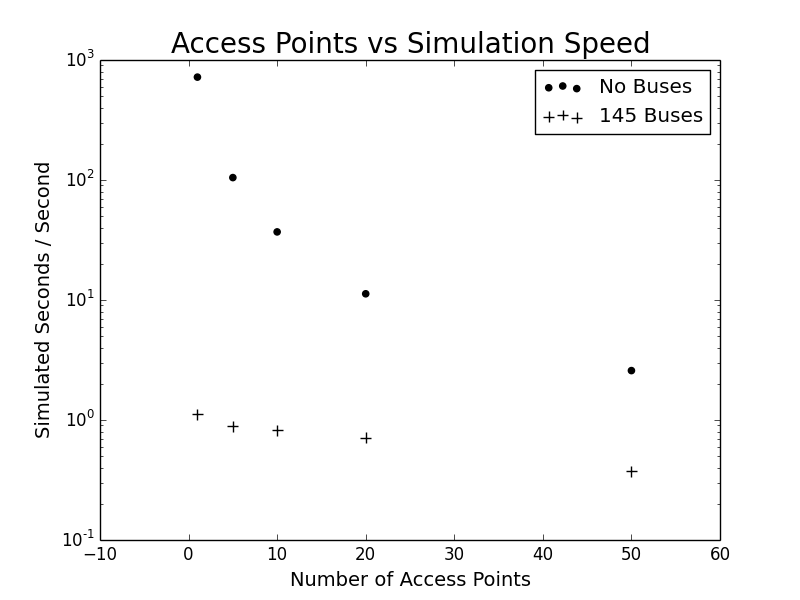
\includegraphics[width=\linewidth]{./images/AP_vs_Simulation_Speed.png}
                    \caption{Simulation speed as a function of the number of access points.}
                    \label{fig:access_points_speed}
                \end{subfigure}%HODOR
                \begin{subfigure}{0.5\textwidth}
                    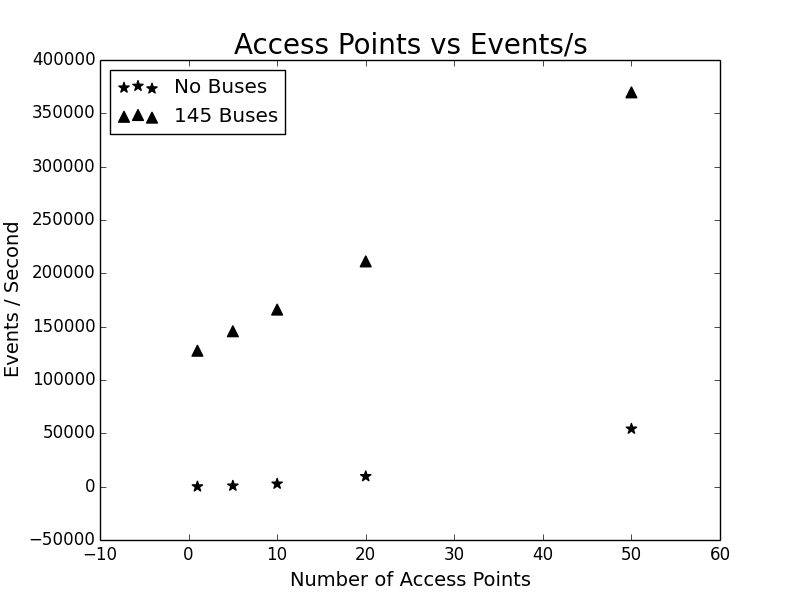
\includegraphics[width=\linewidth]{./images/AP_vs_Events.png}
                    \caption{Number of events as a function of the number of access points.}
                    \label{fig:access_points_events}
                \end{subfigure}
                \caption{Simulation speed and number of events as a function of the number of access points in the simulation. This has been performed for no buses and 145 buses in the simulation.}
                \label{fig:access_points_vs_time_and_events}
            \end{figure}

            When running a full simulation with 50 access points and all 145 buses it took around 3 days to simulate just 1 day. In order to be able to perform all desired experiments and be able to repeat them multiple times in the 6 months which remained at this point, the simulation would have to be improved dramatically. Fortunately, Omnet++ provided a mechanism for this. 

            \emph{MPI}, which stands for Message Passing Interface, is supported by Omnet++~\cite{omnetmpi}. MPI allows simulations to run on multiple cores concurrently. Ordinarily Omnet++ runs on a single core, however if it were to use MPI on a 4 core machine then theoretically it is possible to achieve speed boosts of up to 4 times faster. In practise it is lower due to the message passing overhead, but we would still hope to see the simulation time half. The simulation configuration was configured to allow MPI and some speed tests were run. The results of these tests showed that the simulation was almost twice as slow when using MPI. Further investigation revealed the cause of these problems. 

            
            \centerimage{0.5\textwidth}{./images/Bi-Partite_Network.png}{An example of a suitable place to partition a network, represented by the red line. }{fig:bipartite_network}

            MPI in Omnet++ works extremely well when the networks are cleanly partitioned. For instance, modelling two subnets connected by a switch. Figure~\ref{fig:bipartite_network} shows a logical point to partition the network. In this example, one subnet would run on one core, and the other on a separate core. All communication within the subnet would remain on that core, which would cause no additional overhead. Any communications between subnets would then use MPI. In our model we do not have any clean point to partition. With 145 buses moving all over the city and 50 access points it would be difficult to devise an optimal partition. This problem could be solved using machine learning, however it is beyond the scope of this project. It is theorised that if all entities, that is the buses and access points, were run on a separate core, perhaps using many machines, we may see a performance boost, however this was infeasible. 

            Due to parallelising a single simulation failing, a different approach was taken. Instead of running one simulation on $n$ cores, the decision was made to run $n$ simulations on $n$ cores, essentially one simulation per core. Initial testing was performed on a dual core machine with two simulations. The results showed that the simulations both took more than twice as long as the single test. When this was tested on a quad core machine however, the simulations took slightly less than double the time. This means that the total time to run both simulations was less than running each sequentially, which is a clear improvement. Unfortunately continuous access to this quad core machine was not available and an alternative had to be found. 

            Currently, popular methods of performing large scale computations are to use virtual machines hosted by a third party. Common companies to use for this are \emph{Amazon}, \emph{Rackspace} and \emph{Digital Ocean}. Based on the requirements above, the aim would be to choose multiple instances with 4 cores for the cheapest price. In terms of cost, Digital Ocean was a clear winner, however it was 4 times as expensive to get a 4 core machine as it was to get a 2 core machine. As such, simulations were run on 5 dual core machines. Each machine was given a different random sampling of access points, and all simulations on each machine were run sequentially. This reduced the run time of some tests from over a month to just under a week. 


    \section{Opportunistic Forwarding}\label{simulation_opportunistic_forwarding}

        \tdi{I don't mention how OF helps with packet latency at all.}

        Air quality has been measured using vehicles before such as with the OpenSense project, however these project tend to rely on cellular connectivity for returning the data. Our system does not use cellular connectivity and instead relies on open wifi access points. This method presents certain problems. The main problem being that we have no control over the location of these access points and as such buses may spend a long time out of range of an access point, or indeed may not even come into contact with one at all. Figure~\ref{fig:access_point_map} shows the locations of the 82 access points in Edinburgh we will be using for our simulations. We can see that these access points are clustered around the centre of the city and there are almost none at all at distances of more than 2 miles from the centre. 

        \centerimagewideanywhere{./images/APMap.png}{A map of all 82 open access points which are used in our simulations.}{fig:access_point_map}

        From this image we can see that it is likely that we will run into issues should there be any buses which do not go through the city centre as part of their route. Unfortunately this is the case for at least one particular route. Buses on route 39 do not travel inside the city bypass at all, a boundary which is generally regarded as the bounds of the city. These buses travel around some of the villages in the south of the city. There are no recorded access points outside the bypass. Route 39 is shown in figure~\ref{fig:route_39}.

        \centerimagewideanywhere{./images/Route39.png}{Lothian bus route 39.}{fig:route_39}

        Based on the chemicals discuss in section~\ref{background_air_quality}, we know the data we need to store for each data packet. The total size of each packet is 24 bytes as shown by the packet composition in table~\ref{tab:data_packet}. Research in the first year of this project into creating a physical sensor revealed that the \emph{Arduino Uno} would make a good choice of base component. The reasons for this included its cost, size, and use in similar projects~\cite{arduinoproj1,arduinoproj2,arduinoproj3}. The Uno's main problem however is the limited space for storing data with the standard version having just 32,256 bytes of storage space available~\cite{arduinounospecs}. This means that it can store at most 1,344 packets. With a new measurement every second this amounts to just over 22 minutes of data storage space. A more expensive version has storage space for 10,581 packets, which is just under 3 hours of recording. Ideally we would need at least one full days worth of storage space to ensure that all the recorded data makes it back to the central server since the buses return to a depot within the city at night should they not be in use. In order to ensure that we don't end up with only the last 22 minutes of data for the buses on route 39, and indeed the last 22 minutes before finding an access point on routes which only have minimal access to access points, we need a different method of returning the data.

        \begin{table}
            \centering
            \begin{tabular}{ | c | c |}
                \hline
                Metric & Size (bytes)\\ \hline
                Timestamp & 4 \\
                Bus Id & 2 \\
                \cee{CO_{2}} & 2 \\
                \cee{NO_{x}} & 2 \\
                \cee{O_{3}} & 2 \\
                PM 10 & 2 \\
                PM 2.5 & 2 \\
                Latitude & 4 \\
                Longitude & 4 \\
                \hline
                Total & 24 \\
                \hline
            \end{tabular}
            \caption{The layout of a single data packet.}
            \label{tab:data_packet}
        \end{table}

        The solution for this is known as \emph{opportunistic forwarding}. Opportunistic forwarding consists of buses communicating with one another and passing the data between them so that as much data as possible will be returned to the central server with the lowest possible latency. An example of how this works can be shown using the buses on route 39. On this route there is a straight which the buses on route 40 also traverse. The buses on route 40 however travel into more densely populated areas and come into contact with access points. This can be seen in figure~\ref{fig:route_39_40}. When a bus on route 39 comes into contact with a bus on route 40, the buses exchange information about which will find an access point the soonest and the space they have available. In this case the bus on route 40 will come into contact with an access point first and so will accept the data from the route 39 bus. The bus on route 40 will accept as many packets as it can without causing it to lose any of its own between now and finding an access point. This is achieved by each bus being able to predict when it will come into contact with an access point. In reality this would be achieved by programming this buses with timetables and recording data about the access points they encountered, however since this data is unavailable to this, it is simulated with the current data set. Each bus knows about all 82 access points which are used, but each simulation only uses at most 50 of these. As such, buses may predict that they will encounter an access point which is not present in the simulation. This behaviour is representative of reality in that access points may be missing, however we would expect this to happen to a lesser extent in reality.   

        \centerimagewideanywhere{./images/Route3940.png}{Lothian bus routes 39 and 40.}{fig:route_39_40}

        In a physical implementation of opportunistic forwarding, the standard mechanism would be to use a single radio and switch back and forth between the peer to peer communication mode and the access point detection mode. The reason for doing this is purely cost based. With a simulator we are not limited to this and as such we add a second radio. The addition of a second radio would removes the fraction of a second delay to connecting to an access point when using a single radio, due to the context switch. It also makes it more likely that broadcasts from other buses will be detected. It should be noted that in the simulation, IP address allocation is a complicated procedure and as such the decision was made to limit the number of allocated addresses to less than 255. Due to each bus having two radios we have only 125 buses in our opportunistic forwarding simulations, losing all buses from routes 5 and 37. This will have a negative effect on the performance of opportunistic forwarding, however due to time constraints the decision was made to continue with this method.

        The more important decision to be made is the algorithm which we will use in our model. Lebrun et al. discussed five different algorithms for opportunistic forwarding~\cite{opportunisticforwarding}. These algorithms were \emph{NOTALK}, \emph{BROADCAST}, \emph{Location-based}, \emph{MoVe} and \emph{MOVE-Lookahead}. NOTALK is the base case in which there is no communication between nodes and so will be discounted immediately. BROADCAST is the opposite in that every node exchanges information with every other node it comes into contact with. This method of routing is also known as \emph{epidemic routing}, and was first described by Vahdat et al. in \emph{Epidemic Routing for Partially-Connected Ad Hoc Networks}~\cite{vahdat2000epidemic}. The goals and therefore advantages of epidemic routing, and therefore broadcast BROADCAST, as described by Vahdat et al. are ``i) maximize message delivery rate, ii) minimize message latency, and iii) minimize the total resources consumed in message delivery.'' Using opportunistic forwarding removes one of the main requirements of other routing algorithms which is the assumption that a path to an access point always exists. The price we pay for these advantages however is the large storage space requirements. Obviously this limitation is one which cannot be ignored due to the reasons discussed above and as such we need to discount the BROADCAST algorithm. The MoVe and the MOVE-Lookahead algorithms require much more information than we have available and must be discounted. This leaves us with one algorithm and that is the Location-based algorithm. This algorithm is derived from the BROADCAST algorithm by employing a heuristic. The heuristic is that the algorithm only passes on the data to the other sensor should it reach an access point first. This is the algorithm which was implemented. 

        The algorithm employs the following approach for the broadcasting bus, A:

        \begin{enumerate}
            \item Broadcast first packet in queue to all nearby buses
            \item If we receive a response, remove the packet from the queue and repeat
            \item If we do not receive a response then try again in 0.5 seconds
        \end{enumerate}

        For the receiving bus, B:

        \begin{enumerate}
            \item Compare the time until bus A will reach an access point (AP) to the time that this bus, B, will reach an access point using the information in the packet.
            \item If bus A reaches an AP first then discard this packet and do not respond.
            \item If bus B will reach an AP first then predict how much ``spare'' space bus B will have in it's buffer when reaching the AP:
                \begin{enumerate}
                    \item Calculate time until next AP, $t$.
                    \item Subtract $t$ from space remaining in the queue, $r$, and call this result $s$.
                \end{enumerate}
            \item If $s$ is greater than 0 then accept this packet by adding it to our own queue and broadcasting a response.
        \end{enumerate}

        In order to successfully use this algorithm we need to provide extra information in our packets we send. This extra information includes the time until finding the next access point (4 bytes) and the identifier of the bus the packed \emph{originated} from (2 bytes). This addition of 6 bytes changes our packet size to 30 bytes in total. Which means that each device can no longer hold 1,344 packets and instead can only hold 1,075 packets, or in the case of the larger storage space it changes from 10,581 to 8,465. This is 18 minutes and 141 minutes of data respectively. As will be shown in chapter~\ref{data_gathering_performance} the trade off is justified. 

